\documentclass[conference]{IEEEtran}

\usepackage{cite}
\usepackage{amsmath,amssymb}
\usepackage{booktabs}
\usepackage{array}
\usepackage{siunitx}
\usepackage{pgfplots}
\usepackage{url}
\usepackage[hidelinks]{hyperref}

\pgfplotsset{compat=1.18}
\sisetup{round-mode=places,round-precision=3}
\newcolumntype{L}[1]{>{\raggedright\arraybackslash}p{#1}}
\emergencystretch=2em

\begin{document}

\title{When FLOPs Mislead on PC GPUs: Comparing RTX 3050 and RTX 4060 Inference Energy}

\author{
\IEEEauthorblockN{Aryan Shah}
\IEEEauthorblockA{Texas Academy of Mathematics and Science\\
University of North Texas\\
Denton, TX, USA\\
aryanshah.2431@gmail.com}
\and
\IEEEauthorblockN{Romir Kadiam}
\IEEEauthorblockA{Texas Academy of Mathematics and Science\\
University of North Texas\\
Denton, TX, USA\\
romirkadiam123@gmail.com}
}

\maketitle

\begin{abstract}
This paper reports a Windows CUDA measurement artifact for neural-network
inference energy on two commodity NVIDIA GPUs: an RTX 3050 4GB Laptop GPU and
an RTX 4060 desktop GPU. For each GPU, five image-classification models are
measured in a batch-1 stability run with ten 10-second windows per model and
in a batch-size sweep over batch sizes 1, 4, 8, 16, and 32. The artifact
retains raw \texttt{nvidia-smi} logs and reports GPU-only board energy, not CPU
package energy or wall-plug energy. On the RTX 4060, latency explains most
between-model energy variation ($R^2=0.963$), while FLOPs is weak
($R^2=0.038$). On the RTX 3050 Laptop GPU, latency remains more informative
than FLOPs ($R^2=0.684$ versus $0.011$) but the measurements are noisier. The
batch sweeps show that best per-image energy depends on both model and GPU:
the best batch size ranges from 8 to 32 on the RTX 4060 and from 16 to 32 on
the RTX 3050. These results support a measurement-first PC-GPU benchmark
methodology and show why FLOPs alone is not a reliable energy proxy.
\end{abstract}

\begin{IEEEkeywords}
GPU inference, energy measurement, Windows CUDA, RTX 3050, RTX 4060, PyTorch,
benchmarking
\end{IEEEkeywords}

\section{Introduction}

Model efficiency is often summarized with FLOPs, parameter count, or model
size. Those quantities are useful architecture descriptors, but they do not
directly measure the runtime behavior that determines deployment energy:
operator scheduling, kernel launch overhead, memory movement, batching, and
device utilization. This paper studies that gap with direct Windows CUDA
measurements on two NVIDIA GPUs.

This paper is intentionally separate from the Apple-Silicon CPU-only study in
the companion repository. The Apple paper uses macOS \texttt{powermetrics};
this PC paper uses \texttt{nvidia-smi} GPU-board telemetry. The absolute joules
therefore have a different power boundary and should not be pooled with
package-level or wall-plug measurements. The question here is local and
systems-oriented: under a fixed Windows CUDA artifact, do architecture proxies
such as FLOPs track measured GPU-only inference energy?

The current contributions are:
\begin{itemize}
\item A reproducible Windows CUDA workflow with raw \texttt{nvidia-smi} logs,
environment metadata, randomized model order, and confidence intervals.
\item Batch-1 energy measurements for five models on an RTX 3050 Laptop GPU
and an RTX 4060 desktop GPU.
\item A comparison showing that latency is a stronger predictor of GPU-only
energy than FLOPs on both GPUs, though the strength differs by system.
\item Batch-size sweeps showing that per-image energy changes by up to
$20.1\times$ and that the best batch size is model- and GPU-dependent.
\item A clear boundary statement: the artifact measures GPU board energy only,
not CPU package energy or whole-system wall power.
\end{itemize}

\section{Related Work and Motivation}

Efficient model families such as MobileNet, EfficientNet, and residual
networks make different tradeoffs among depthwise convolution, channel width,
residual connectivity, and operator mix \cite{mobilenetv2,efficientnet,resnet}.
FLOPs and parameters are portable, but they do not capture kernel choice,
memory traffic, launch overhead, or how well a given GPU is utilized.
Prior model-efficiency studies have similarly shown that arithmetic count,
parameter count, memory footprint, and measured speed can rank networks
differently in practice \cite{canziani}. At the hardware level, energy cost is
also shaped by memory movement and data movement, not just arithmetic
operations \cite{horowitz}.

Systems benchmarking work therefore emphasizes measured deployment behavior.
MLPerf Inference separates latency-oriented and throughput-oriented scenarios
rather than assuming one number characterizes all deployments \cite{mlperf}.
NVIDIA's \texttt{nvidia-smi} and NVML tooling expose useful GPU telemetry, but
that telemetry is device-level rather than whole-system energy \cite{nvidiasmi}.
This paper follows that measurement-first approach for a small, auditable
PC-GPU artifact. The broader motivation is also environmental and operational:
energy-aware machine learning work has argued that reporting compute and energy
costs is necessary for transparent model evaluation \cite{strubell}.

\section{Measurement Scope}

Table~\ref{tab:env} summarizes the two systems. Both runs use CUDA, float32,
batch size 1 for the main stability measurement, an input shape of
$1\times3\times224\times224$, and the same five model definitions. The RTX
3050 run uses Python 3.8.10 and PyTorch 2.4.1+cu124; the RTX 4060 run uses
Python 3.11.9 and PyTorch 2.11.0+cu128. Because software versions differ, the
paper treats the systems as deployment measurements rather than as a controlled
GPU microbenchmark.

\begin{table}[t]
\centering
\caption{Windows CUDA measurement environments.}
\label{tab:env}
\tiny
\begin{tabular}{@{}L{0.24\linewidth}L{0.27\linewidth}L{0.29\linewidth}@{}}
\toprule
Component & RTX 3050 system & RTX 4060 system\\
\midrule
GPU & RTX 3050 4GB Laptop GPU & RTX 4060\\
CPU & Intel64 Model 186 & Intel64 Model 191\\
Python / PyTorch & 3.8.10 / 2.4.1+cu124 & 3.11.9 / 2.11.0+cu128\\
Power backend & \texttt{nvidia-smi}, GPU-only & \texttt{nvidia-smi}, GPU-only\\
Main protocol & 10 windows/model, 10 s/window & 10 windows/model, 10 s/window\\
Batch sweep & $B=1,4,8,16,32$ & $B=1,4,8,16,32$\\
\bottomrule
\end{tabular}
\end{table}

The repository has four active data directories, one batch-1 directory and one
batch-sweep directory for each GPU. Each contains the summary CSV, trial CSV,
environment JSON, and raw power logs for the corresponding run.

\section{Power Logging}

The measurement script first tries the structured \texttt{nvidia-smi} CSV query
for instantaneous power. When that field is unavailable, the script falls back
to parsing the raw \texttt{nvidia-smi -q -d POWER} text while preserving the
raw log. Energy per inference is computed as
\begin{equation}
E_{\mathrm{gpu,inf}} =
\frac{\bar{P}_{\mathrm{gpu}}\Delta t}{N},
\end{equation}
where $\bar{P}_{\mathrm{gpu}}$ is mean sampled GPU board power, $\Delta t$ is
the measured window duration, and $N$ is the number of completed inferences.
For batch sweeps, per-image energy is
\begin{equation}
E_{\mathrm{gpu,img}} =
\frac{\bar{P}_{\mathrm{gpu}}\Delta t}{NB},
\end{equation}
where $B$ is batch size. These quantities are GPU-only and should not be read
as CPU package or wall-plug energy.

\begin{table}[t]
\centering
\caption{Measurement validity checks.}
\label{tab:checks}
\scriptsize
\begin{tabular}{@{}L{0.34\linewidth}L{0.55\linewidth}@{}}
\toprule
Risk & Check or mitigation\\
\midrule
Startup overhead & discard 10 warmup inferences before each window\\
Order effects & randomize model order with recorded seed\\
Power parser failure & retain raw \texttt{nvidia-smi} output for every window\\
Missing samples & require nonzero parsed windows before energy claims\\
Boundary confusion & label all energy as GPU-only\\
Batch ambiguity & report batch size and per-image metrics separately\\
\bottomrule
\end{tabular}
\end{table}

\section{Batch-1 Results}

Table~\ref{tab:batch1} gives the main batch-1 energy measurements. Every model
has 10 parsed energy windows on both GPUs. The RTX 4060 is much faster, with
2.6--3.2$\times$ lower latency than the RTX 3050 Laptop GPU, but it also draws
substantially higher average board power. As a result, the RTX 4060 uses more
GPU-board energy per batch-1 inference for every model in this artifact.

\begin{table*}[t]
\centering
\caption{Batch-1 Windows CUDA inference results. Energy is GPU-only from
\texttt{nvidia-smi} power samples.}
\label{tab:batch1}
\scriptsize
\begin{tabular}{@{}lrrrrrrrr@{}}
\toprule
Model & FLOPs & \multicolumn{3}{c}{RTX 3050 Laptop} &
\multicolumn{3}{c}{RTX 4060} & 4060/3050\\
\cmidrule(lr){3-5}\cmidrule(lr){6-8}
 & (G) & Energy (J) & Lat. (ms) & Power (W) &
 Energy (J) & Lat. (ms) & Power (W) & Energy\\
\midrule
MobileNetV3-S & 0.113 & 0.107 & 13.55 & 8.43 & 0.236 & 4.31 & 54.91 & 2.21\\
MobileNetV2 & 0.602 & 0.109 & 11.31 & 10.21 & 0.248 & 4.38 & 56.67 & 2.27\\
ResNet-18 & 3.628 & 0.102 & 6.01 & 17.84 & 0.165 & 2.02 & 81.45 & 1.61\\
Tiny-ViT-5M & 2.331 & 0.211 & 18.20 & 12.63 & 0.415 & 6.95 & 59.68 & 1.96\\
EffNet-B0 & 0.772 & 0.171 & 18.60 & 9.96 & 0.383 & 6.80 & 56.35 & 2.24\\
\bottomrule
\end{tabular}
\end{table*}

The key point is not that one GPU is universally ``better'' in absolute
joules. The power boundary is GPU board power only, and the systems differ in
driver stack, PyTorch version, and device class. The key point is that FLOPs
does not determine the energy order on either system. ResNet-18 has the
largest FLOP count but is the lowest-energy batch-1 model on both GPUs.
EfficientNet-B0 has far fewer FLOPs than ResNet-18 but consumes more energy on
both systems.

\begin{table}[t]
\centering
\caption{Batch-1 95\% confidence intervals for GPU-only energy. Values are
joules per inference.}
\label{tab:ci}
\scriptsize
\begin{tabular}{@{}lrr@{}}
\toprule
Model & RTX 3050 & RTX 4060\\
\midrule
MobileNetV3-S & [0.061, 0.152] & [0.232, 0.241]\\
MobileNetV2 & [0.089, 0.129] & [0.245, 0.252]\\
ResNet-18 & [0.084, 0.121] & [0.162, 0.167]\\
Tiny-ViT-5M & [0.167, 0.256] & [0.410, 0.419]\\
EffNet-B0 & [0.123, 0.219] & [0.379, 0.388]\\
\bottomrule
\end{tabular}
\end{table}

The intervals reveal a measurement difference between the systems. The RTX
4060 run has tight intervals because the board-power samples and inference
counts are stable across windows. The RTX 3050 Laptop GPU run is usable, with
all windows parsed, but it is visibly noisier. MobileNetV3-Small and
EfficientNet-B0 show especially wide intervals, so their exact batch-1 energy
values should be interpreted more cautiously than the RTX 4060 values. This
does not change the qualitative ranking result: FLOPs remains a poor proxy,
and ResNet-18 remains low energy despite having the largest FLOP count.

\begin{table}[t]
\centering
\caption{Univariate predictors of batch-1 GPU-only energy across five model
means.}
\label{tab:predictors}
\small
\begin{tabular}{lrr}
\toprule
Predictor & RTX 3050 & RTX 4060\\
\midrule
Latency (ms/inference) & 0.684 & 0.963\\
FLOPs (G) & 0.011 & 0.038\\
Parameters (M) & 0.190 & 0.020\\
\bottomrule
\end{tabular}
\end{table}

\begin{figure}[t]
\centering
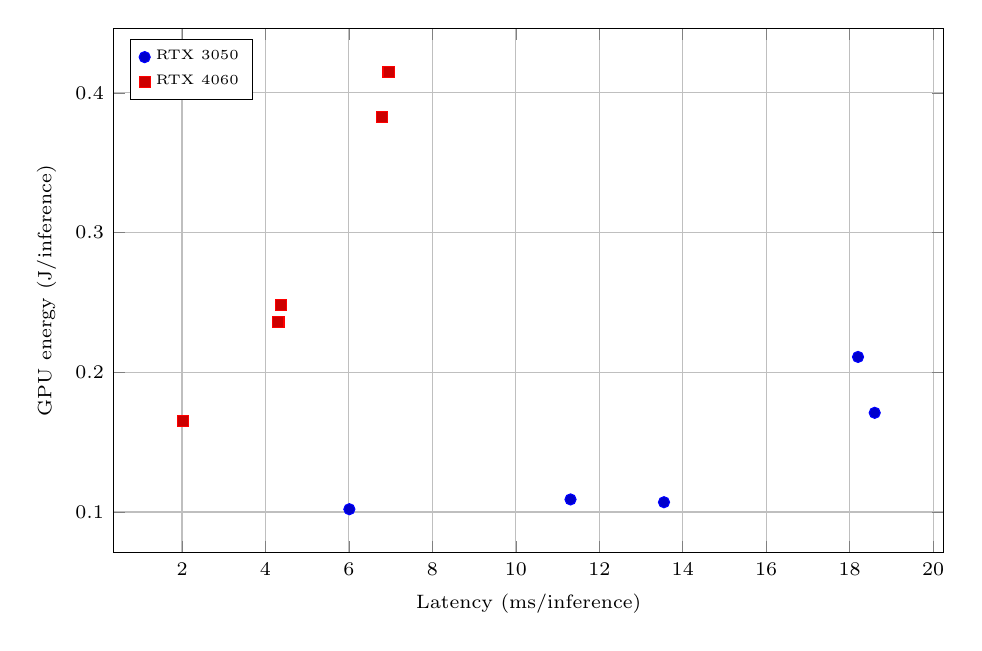
\begin{tikzpicture}
\begin{axis}[
    width=\linewidth,
    height=0.68\linewidth,
    xlabel={Latency (ms/inference)},
    ylabel={GPU energy (J/inference)},
    grid=both,
    tick label style={font=\scriptsize},
    label style={font=\scriptsize},
    legend style={font=\tiny, at={(0.02,0.98)}, anchor=north west},
]
\addplot+[only marks] coordinates {
    (13.55,0.107) (11.31,0.109) (6.01,0.102) (18.20,0.211) (18.60,0.171)
};
\addlegendentry{RTX 3050}
\addplot+[only marks] coordinates {
    (4.31,0.236) (4.38,0.248) (2.02,0.165) (6.95,0.415) (6.80,0.383)
};
\addlegendentry{RTX 4060}
\end{axis}
\end{tikzpicture}
\caption{Batch-1 GPU-only energy versus latency. Latency is informative on
both GPUs, but the RTX 3050 measurements are noisier.}
\label{fig:energy-latency}
\end{figure}

\begin{figure}[t]
\centering
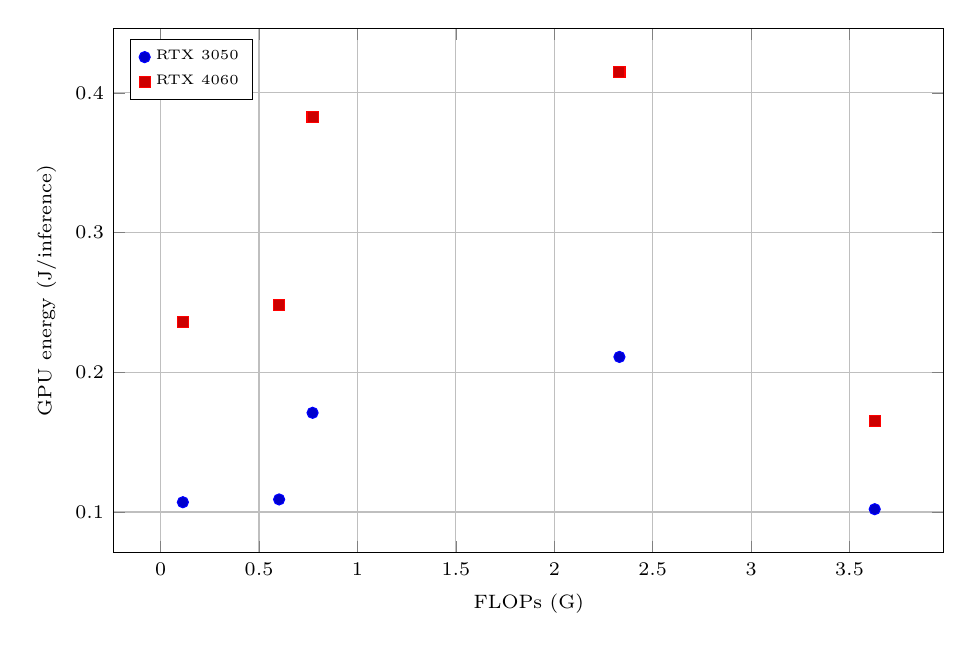
\begin{tikzpicture}
\begin{axis}[
    width=\linewidth,
    height=0.68\linewidth,
    xlabel={FLOPs (G)},
    ylabel={GPU energy (J/inference)},
    grid=both,
    tick label style={font=\scriptsize},
    label style={font=\scriptsize},
    legend style={font=\tiny, at={(0.02,0.98)}, anchor=north west},
]
\addplot+[only marks] coordinates {
    (0.113,0.107) (0.602,0.109) (3.628,0.102) (2.331,0.211) (0.772,0.171)
};
\addlegendentry{RTX 3050}
\addplot+[only marks] coordinates {
    (0.113,0.236) (0.602,0.248) (3.628,0.165) (2.331,0.415) (0.772,0.383)
};
\addlegendentry{RTX 4060}
\end{axis}
\end{tikzpicture}
\caption{Batch-1 GPU-only energy versus FLOPs. ResNet-18 has the largest FLOP
count but is the lowest-energy model on both GPUs.}
\label{fig:energy-flops}
\end{figure}

\begin{table}[t]
\centering
\caption{Cross-GPU batch-1 deltas. Latency speedup is RTX 3050 latency divided
by RTX 4060 latency.}
\label{tab:deltas}
\scriptsize
\begin{tabular}{@{}lrr@{}}
\toprule
Model & 4060/3050 energy & 4060 latency speedup\\
\midrule
MobileNetV3-S & 2.21 & 3.15\\
MobileNetV2 & 2.27 & 2.58\\
ResNet-18 & 1.61 & 2.97\\
Tiny-ViT-5M & 1.96 & 2.62\\
EffNet-B0 & 2.24 & 2.73\\
\bottomrule
\end{tabular}
\end{table}

Table~\ref{tab:deltas} makes the power-latency tradeoff explicit. The RTX 4060
is between 2.58$\times$ and 3.15$\times$ faster at batch 1, but it uses
1.61$\times$ to 2.27$\times$ more GPU-board energy per inference. This is not
a contradiction: the faster GPU operates at a much higher board-power level.
It also means that an energy paper should avoid collapsing the result into a
single winner. The energy-minimizing hardware under batch-1 GPU-board energy is
not necessarily the latency-minimizing hardware, and neither is necessarily the
best throughput hardware once batching is allowed.

\section{Batch-Size Sweeps}

Batching changes the denominator of the energy calculation. A larger batch can
draw more board power while still reducing per-image energy if throughput
increases enough. Table~\ref{tab:bestbatch} reports the best observed batch
size for each model and GPU. Both systems show large gains over batch 1, but
the best batch size is not constant across models or GPUs.

\begin{table*}[t]
\centering
\caption{Best observed batch size by GPU-only energy per image. Gain compares
batch size 1 with the best per-image energy in the sweep.}
\label{tab:bestbatch}
\scriptsize
\begin{tabular}{@{}lrrrrrrrr@{}}
\toprule
Model & \multicolumn{4}{c}{RTX 3050 Laptop} &
\multicolumn{4}{c}{RTX 4060}\\
\cmidrule(lr){2-5}\cmidrule(lr){6-9}
 & Best $B$ & E/img & Images/s & Gain &
 Best $B$ & E/img & Images/s & Gain\\
\midrule
MobileNetV3-S & 32 & 0.0130 & 1111 & 20.1 & 32 & 0.0127 & 7495 & 18.6\\
MobileNetV2 & 16 & 0.0523 & 280 & 3.8 & 8 & 0.0451 & 2012 & 5.4\\
ResNet-18 & 32 & 0.0479 & 311 & 2.9 & 16 & 0.0464 & 2114 & 3.3\\
Tiny-ViT-5M & 16 & 0.1245 & 120 & 3.3 & 8 & 0.1039 & 958 & 3.9\\
EffNet-B0 & 16 & 0.0690 & 214 & 4.5 & 16 & 0.0668 & 1419 & 5.8\\
\bottomrule
\end{tabular}
\end{table*}

\begin{table*}[t]
\centering
\caption{GPU-only energy per image across the batch sweeps. Values are joules
per image.}
\label{tab:batchcurve}
\tiny
\begin{tabular}{@{}lrrrrrrrrrr@{}}
\toprule
Model & \multicolumn{5}{c}{RTX 3050 Laptop} &
\multicolumn{5}{c}{RTX 4060}\\
\cmidrule(lr){2-6}\cmidrule(lr){7-11}
 & B1 & B4 & B8 & B16 & B32 & B1 & B4 & B8 & B16 & B32\\
\midrule
MobileNetV3-S & 0.2608 & 0.0824 & 0.0497 & 0.0318 & 0.0130 & 0.2354 & 0.0634 & 0.0352 & 0.0213 & 0.0127\\
MobileNetV2 & 0.2008 & 0.1003 & 0.0663 & 0.0523 & 0.0581 & 0.2438 & 0.0769 & 0.0451 & 0.0525 & 0.0560\\
ResNet-18 & 0.1403 & 0.0786 & 0.0589 & 0.0498 & 0.0479 & 0.1545 & 0.0582 & 0.0499 & 0.0464 & 0.0496\\
Tiny-ViT-5M & 0.4102 & 0.1710 & 0.1424 & 0.1245 & 0.1284 & 0.4102 & 0.1333 & 0.1039 & 0.1076 & 0.1076\\
EffNet-B0 & 0.3092 & 0.1567 & 0.0955 & 0.0690 & 0.0725 & 0.3846 & 0.1184 & 0.0674 & 0.0668 & 0.0720\\
\bottomrule
\end{tabular}
\end{table*}

\begin{table}[t]
\centering
\caption{Best-batch mean GPU board power. Values are watts at the
energy-minimizing batch size in Table~\ref{tab:bestbatch}.}
\label{tab:bestpower}
\scriptsize
\begin{tabular}{@{}lrr@{}}
\toprule
Model & RTX 3050 & RTX 4060\\
\midrule
MobileNetV3-S & 14.4 & 95.0\\
MobileNetV2 & 14.6 & 90.7\\
ResNet-18 & 14.9 & 98.0\\
Tiny-ViT-5M & 15.0 & 99.6\\
EffNet-B0 & 14.8 & 94.8\\
\bottomrule
\end{tabular}
\end{table}

Table~\ref{tab:batchcurve} shows why the best-batch result should not be
reduced to a single global recommendation. MobileNetV3-Small continues to
benefit through batch 32 on both GPUs. MobileNetV2 reaches its best energy at
batch 16 on the RTX 3050 but at batch 8 on the RTX 4060. Tiny-ViT-5M also
peaks earlier on the RTX 4060 than on the RTX 3050. These differences are
plausible because the two GPUs have different power envelopes and utilization
behavior, and they reinforce the need to report batch size explicitly.

\begin{figure}[t]
\centering
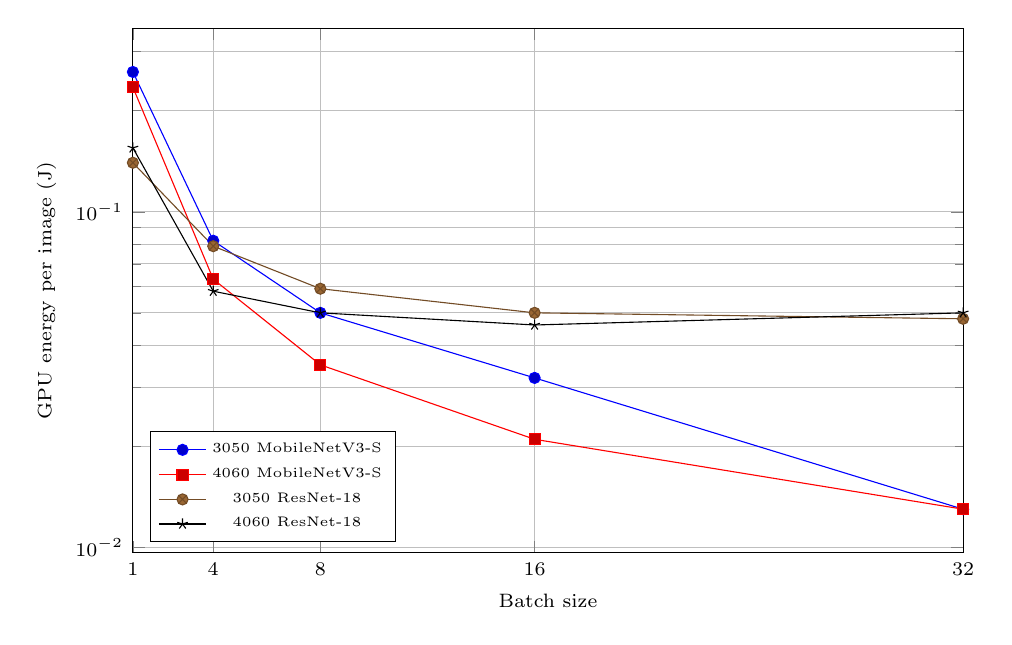
\begin{tikzpicture}
\begin{axis}[
    width=\linewidth,
    height=0.68\linewidth,
    ymode=log,
    xlabel={Batch size},
    ylabel={GPU energy per image (J)},
    xmin=1, xmax=32,
    xtick={1,4,8,16,32},
    grid=both,
    tick label style={font=\scriptsize},
    label style={font=\scriptsize},
    legend style={font=\tiny, at={(0.02,0.02)}, anchor=south west},
]
\addplot coordinates {(1,0.261) (4,0.082) (8,0.050) (16,0.032) (32,0.013)};
\addlegendentry{3050 MobileNetV3-S}
\addplot coordinates {(1,0.235) (4,0.063) (8,0.035) (16,0.021) (32,0.013)};
\addlegendentry{4060 MobileNetV3-S}
\addplot coordinates {(1,0.140) (4,0.079) (8,0.059) (16,0.050) (32,0.048)};
\addlegendentry{3050 ResNet-18}
\addplot coordinates {(1,0.155) (4,0.058) (8,0.050) (16,0.046) (32,0.050)};
\addlegendentry{4060 ResNet-18}
\end{axis}
\end{tikzpicture}
\caption{Example batch-sweep curves. Batching helps both GPUs, but the energy
curve and optimum are model- and device-dependent.}
\label{fig:batch-energy}
\end{figure}

For throughput-oriented use, the RTX 4060 delivers much higher image rate at
similar or slightly lower best per-image GPU energy. For example, MobileNetV3
reaches nearly the same best per-image energy on both GPUs, but the RTX 4060
achieves roughly 6.7$\times$ the image rate at that point. This illustrates why
energy, latency, and throughput should be reported together.

\section{Discussion}

The two-GPU artifact strengthens the original single-GPU result. FLOPs is weak
on both systems, while latency is more predictive. However, the RTX 3050 result
also shows that latency is not a universal law: its $R^2$ is lower and the
batch-1 confidence intervals are wider. That difference is useful rather than
embarrassing, because it shows that a publishable benchmark should expose
system-specific behavior rather than forcing all devices into one proxy.

The RTX 4060 is consistently faster, but it draws much more board power. In
batch-1 mode, the power increase is large enough that the RTX 4060 consumes
more GPU-board energy per inference for these five models. Under batching, the
RTX 4060 becomes more attractive for throughput-oriented operation because its
image rate increases sharply while best per-image energy is similar to or
lower than the RTX 3050. This is exactly why batch size is a first-order
experimental condition, not an implementation detail.

The comparison also separates two meanings of ``efficient.'' For a
latency-constrained interactive system, the RTX 4060 is preferable because it
finishes each request much faster. For a strict GPU-board-energy-per-request
metric at batch 1, the RTX 3050 Laptop GPU is lower energy in this artifact
because its board power is much lower. For buffered throughput, the answer
changes again: the RTX 4060 can process far more images per second at nearly
the same best per-image energy. A paper that reports only FLOPs, or only
batch-1 latency, would miss those distinctions.

\section{Protocol for Added Systems}

The artifact is structured so another Windows CUDA system can be added without
changing the paper workflow. A contributed system should include the complete
output directory from the measurement script, not just the summary CSV. The
minimum required files are \texttt{pc\_inference\_trials.csv},
\texttt{pc\_inference\_summary.csv},
\texttt{pc\_measurement\_environment.json}, and the complete
\texttt{raw\_power/} directory. The environment JSON is important because GPU
model, driver behavior, CUDA version, PyTorch version, and Python version can
all change measured latency and power.

\begin{table}[t]
\centering
\caption{Minimum metadata needed for each additional PC-GPU system.}
\label{tab:metadata}
\scriptsize
\begin{tabular}{@{}L{0.34\linewidth}L{0.55\linewidth}@{}}
\toprule
Field & Reason\\
\midrule
GPU and driver & power telemetry support differs by device and driver\\
CPU model & dispatch overhead is outside GPU energy but affects runtime\\
PyTorch/CUDA versions & kernel selection can change latency and power\\
Power backend & distinguishes GPU-only, CPU package, and wall power\\
Batch sizes & separates low-latency serving from throughput operation\\
Raw logs & allows parser failures and missing samples to be audited\\
\bottomrule
\end{tabular}
\end{table}

For future systems, the batch-1 run should be collected first because it gives
the cleanest predictor comparison. The batch sweep should then be collected
with the same set $B\in\{1,4,8,16,32\}$ when memory permits. Runs with zero
parsed power samples should be retained as latency data but excluded from
energy claims until the parser or power backend is fixed.

\section{Measurement Implementation}

The measurement script uses a windowed workload rather than timing one
inference at a time. A single inference is too short for robust power sampling,
especially on Windows where \texttt{nvidia-smi} reports power at a coarser
cadence than CUDA kernel execution. Each trial therefore runs the model
repeatedly for a fixed wall-clock window, counts completed inferences, samples
GPU power in parallel, and divides total estimated GPU energy by the number of
completed inferences.

\begin{table}[t]
\centering
\caption{Windowed measurement loop used by the artifact.}
\label{tab:algorithm}
\scriptsize
\begin{tabular}{@{}L{0.09\linewidth}L{0.82\linewidth}@{}}
\toprule
Step & Action\\
\midrule
1 & Load the five model definitions and fix input shape, device, dtype, and seed.\\
2 & Randomize model order for each repeat to reduce ordering effects.\\
3 & Run warmup inferences before each measured window.\\
4 & Start \texttt{nvidia-smi} logging and repeatedly execute forward passes for
the target window duration.\\
5 & Store raw power text, completed inference count, elapsed time, latency, and
parsed sample count for the trial.\\
6 & Aggregate trial rows into per-model summary rows with means, standard
deviations, standard errors, and 95\% confidence intervals.\\
\bottomrule
\end{tabular}
\end{table}

This design has two practical advantages. First, it keeps the energy value
auditable: if a summary row looks wrong, the corresponding trial rows and raw
power logs can be inspected directly. Second, it makes failed telemetry visible
instead of silently producing zeros. The paper only uses rows with nonzero
parsed energy windows for energy claims. Latency values from failed power runs
can still be useful, but they should not be mixed with direct energy results.

The batch sweep reuses the same loop but changes the input batch dimension.
The summary CSV reports per-forward values, while the trial CSV also records
per-image latency and energy. This distinction is necessary because a batch-32
forward pass performs 32 image inferences. In the paper, batch comparisons use
per-image values; batch-1 predictor comparisons use the longer batch-1
stability runs.

\section{Measurement Quality}

The RTX 3050 Laptop GPU run is valid but visibly noisier than the RTX 4060 run.
Table~\ref{tab:relci} reports relative confidence-interval width, computed as
$(\mathrm{CI}_{high}-\mathrm{CI}_{low})/\bar{E}$. This quantity is useful
because it makes uncertainty comparable across models with different absolute
energy values.

\begin{table}[t]
\centering
\caption{Relative width of the 95\% energy confidence interval. Lower is
better.}
\label{tab:relci}
\scriptsize
\begin{tabular}{@{}lrr@{}}
\toprule
Model & RTX 3050 & RTX 4060\\
\midrule
MobileNetV3-S & 85.0\% & 3.4\%\\
MobileNetV2 & 36.4\% & 2.9\%\\
ResNet-18 & 35.6\% & 2.7\%\\
Tiny-ViT-5M & 42.3\% & 2.1\%\\
EffNet-B0 & 56.1\% & 2.4\%\\
\bottomrule
\end{tabular}
\end{table}

This table is important for interpretation. The RTX 3050 data should be used
for broad patterns: FLOPs is weak, latency is more informative, and batching
changes per-image energy substantially. It should not be overread as precise
ranking evidence when confidence intervals overlap. The RTX 4060 data support
more precise model-to-model comparisons because every relative interval is
below 4\%. A stronger future artifact would repeat the RTX 3050 run, align the
software stack with the RTX 4060 system, and compare \texttt{nvidia-smi}
against NVML or wall-meter measurements.

\section{Reproducibility and Validity}

Each run includes a trial CSV, summary CSV, environment JSON, and raw power log
directory. The paper uses a summary value only when all model windows have
nonzero parsed power samples. The RTX 3050 and RTX 4060 batch-1 runs both pass
that check with 10 parsed windows per model. The raw logs are retained so that
parser failures or driver-specific power-field differences can be audited.

There are still important limits. The artifact measures GPU board energy, not
whole-PC wall power. CPU dispatch, host memory, storage, display, cooling, and
power-supply losses are outside the boundary. The two systems also differ in
software stack, so the results should be read as deployment measurements, not
as a pure architectural comparison of GPU silicon. Finally, the five-model
regressions are descriptive; broader claims require more GPUs, repeated
software versions, and ideally an external power meter for cross-checking.

\section{Artifact Availability}

The organized repository stores the current paper in \texttt{paper/}. The RTX
3050 data are under \texttt{data/rtx3050\_batch1\_main/} and
\texttt{data/rtx3050\_batch\_sweep/}. The RTX 4060 data are under
\texttt{data/rtx4060\_batch1\_main/} and
\texttt{data/rtx4060\_batch\_sweep/}. The original submitted RTX 3050 bundle
is retained as \texttt{aryan.zip}. Each active directory includes the trial
CSV, summary CSV, environment JSON, and raw power logs.

\section{Conclusion}

Across two Windows CUDA systems, FLOPs is a poor proxy for GPU-only inference
energy. Latency is more informative on both GPUs, but the strength of that
relationship is system-dependent. Batch size also changes the energy picture:
best per-image energy varies by model and GPU, and the RTX 4060's higher board
power is offset by much higher throughput in batched operation. The result is a
more credible PC-GPU paper than a single-device study because it shows both a
common pattern and a device-specific difference.

\begin{thebibliography}{1}

\bibitem{resnet}
K.~He, X.~Zhang, S.~Ren, and J.~Sun, ``Deep residual learning for image
recognition,'' in \emph{Proc. IEEE Conference on Computer Vision and Pattern
Recognition}, 2016.

\bibitem{mobilenetv2}
M.~Sandler, A.~Howard, M.~Zhu, A.~Zhmoginov, and L.-C. Chen,
``MobileNetV2: Inverted residuals and linear bottlenecks,'' in \emph{Proc.
IEEE Conference on Computer Vision and Pattern Recognition}, 2018.

\bibitem{efficientnet}
M.~Tan and Q.~Le, ``EfficientNet: Rethinking model scaling for convolutional
neural networks,'' in \emph{Proc. International Conference on Machine
Learning}, 2019.

\bibitem{canziani}
A.~Canziani, A.~Paszke, and E.~Culurciello, ``An analysis of deep neural
network models for practical applications,'' arXiv:1605.07678, 2016.

\bibitem{horowitz}
M.~Horowitz, ``1.1 Computing's energy problem (and what we can do about it),''
in \emph{Proc. IEEE International Solid-State Circuits Conference}, 2014.

\bibitem{mlperf}
V.~J. Reddi et al., ``MLPerf Inference Benchmark,'' in \emph{Proc. ACM/IEEE
International Symposium on Computer Architecture}, 2020.

\bibitem{nvidiasmi}
NVIDIA, ``NVIDIA System Management Interface,'' available:
\url{https://developer.nvidia.com/system-management-interface}.

\bibitem{strubell}
E.~Strubell, A.~Ganesh, and A.~McCallum, ``Energy and policy considerations
for deep learning in NLP,'' in \emph{Proc. ACL}, 2019.

\end{thebibliography}

\end{document}
